\chapter{Le développement de jeux vidéos}

\label{chap.dev_jv}
Dans ce chapitre, nous pr\'esentons les concepts cl\'es
li\'es au d\'eveloppement de jeux vid\'eos, notamment, les \'etapes de
cr\'eation d'un jeu, la distinction entre exploitation et exploration,
les moteurs de jeux, les types de mécaniques de jeu.
%
Mais tout d'abord, nous pr\'esentons une notion qui revient
souvent dans les sections qui suivent, soit celle de mécanique de jeu.



\section{La notion de mécanique de jeu}

La mécanique d'un jeu vidéo est la façon dont le joueur se servira des éléments de l'environnement pour progresser vers le but du jeu.
Le joueur définit une stratégie et met en place les éléments comme il le souhaite afin de remplir les objectifs du jeu auquel il joue.
Dans un MMORPG --- \emph{Massive Multiplayer Online Role-Playing Game}, un genre de jeu vidéo défini \`a la Section~\ref{MMORPG} --- la mécanique de jeu pourrait donner lieu \`a un sc\'enario comme le suivant :
\begin{itemize}
    \item Je suis un guerrier;
    \item Je vais devoir me battre contre un \emph{boss}
\footnote{Dans un jeu vid\'eo, un \emph{boss} est un type de créature puissante qui représente généralement un défi important, dont l'affrontement marque une étape décisive de l'histoire ou d'une zone. Un affrontement avec un \emph{boss} génère plus d'expérience et permet de ramasser des objets plus rares qu'un affrontement avec une créature normale.}
% 
      effectuant des attaques de glace;
    \item Ce \emph{boss} est sensible aux attaques de feu;
    \item En toute logique, je dois équiper mon personnage en conséquence, donc 
     je m'équipe d'une armure A me défendant contre la glace et d'une arme A faisant des dégâts de feu.
\end{itemize}
Rolling et Morris~\cite{Rollings2004} avancent qu'une mécanique de jeu doit éviter d'être triviale afin de pouvoir laisser le choix à un joueur d'adapter sa stratégie en fonction de nombreuses caractéristiques.
Cela peut amener à des choix qui semblent moins évidents mais qui deviennent plus efficaces, en fonction des éléments réunis dans le combat.
Prenon le cas précédent de notre \emph{boss} de glace.
\begin{itemize}
    \item Le joueur sait que le \emph{boss} a une seule attaque de glace dévastatrice;
    \item Sur un équipement, disons Armure B, il a la possibilité d'annuler cette capacité du \emph{boss};
    \item Cette Armure B possèdes des caract\'eristiques de protection contre la foudre et d'augmentation de dégâts.
\end{itemize}
Le joueur se retrouve alors devant deux choix qui peuvent tous deux sembler corrects :
\begin{enumerate}
    \item Équiper l'Armure A afin de se protéger et limiter les dégâts du \emph{boss};
    \item Équiper l'Armure B, annuler l'attaque de glace du \emph{boss}, tuer le \emph{boss} plus rapidement avec l'augmentation de ses dégâts. 
\end{enumerate}
Les deux cas sont à prendre en compte par le joueur car ils ont chacun leurs avantages et leurs inconvénients.
C'est ce type de choix, selon Rolling et Morris~\cite{Rollings2004}, qui apporte un \emph{gameplay} riche et intéressant~;  
ils avancent même que l'équilibre entre plusieurs mécaniques de jeu est crucial pour l'int\'er\^et d'un jeu.

Une option présente dans un jeu mais n'ayant aucun intérêt \`a être jouée est une erreur de \emph{game design}, que Rolling et Morris qualifient de <<~stratégie dominée~>>. 
Dans la même optique, une option présente qui semble être la seule viable ou supérieure à toutes les autres, peu importe les facteurs extérieurs, est qualifiée de <<~stratégie dominante~>>.

Ainsi, un type de mécanique de jeu réellement plus puissant que les autres enlèverait une partie du <<~\emph{fun}~>> ressenti par le joueur, car ce ne serait plus une question de choix, mais juste une question de calculs.
Un joueur souhaitant faire le choix d'une stratégie moins évidente et moins évidente serait désavantagé par une mécanique de jeu trop forte par rapport aux autres.
C'est ce que Rolling et Morris~\cite{Rollings2004} qualifient de <<~problème de la stratégie dominante~>>. 
Afin de contrer ce problème, ils avancent que laisser une marge de manoeuvre plus grande aux joueurs permet d'éviter ce souci en leur permettant de construire leurs propres stratégies.
Ils considèrent donc que <<~Un jeu bien conçu ne devrait pas contenir d'options qui ne valent pas la peine d'être jouées~>>~\cite{Rollings2004}.

Par contre, ces m\^emes auteurs précisent qu'une option de mécanique de jeu n'est pas un simple choix logique.
Une mécanique de jeu doit être réfléchie et composée de nombreuses règles afin de pouvoir permettre la présence de plusieurs stratégies viables dans un même cas donné.
%
Chaque choix doit avoir ses avantages et ses inconvénients propres afin que le joueur puisse faire un choix en fonction de ses connaissances du jeu et des connaissances de son environnement.
Ce choix, s'il comprend plusieurs solutions viables à plusieurs niveaux, est alors un choix \emph{non trivial}.
Cette liberté de choix crée une sensation de plaisir pour le joueur.
%
La réussite de la stratégie choisie par le joueur entraîne alors une satisfaction pour ce joueur.
L'échec, quant à lui, crée une frustration qui entraîne le joueur vers une nouvelle phase de réflexion pour améliorer sa stratégie.


\section{Les étapes de création d'un jeu vid\'eo}
\label{prob.etapes}
%Conférence Ubisoft a l'UQAM
\begin{figure}[H]
    \centering
    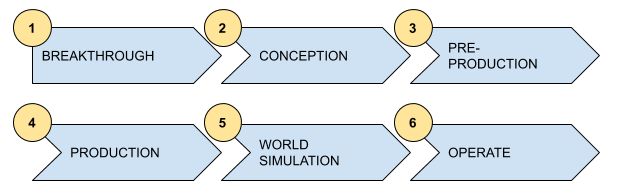
\includegraphics[width=14cm]{10_img/production_stages.png} 
    \caption{Les étapes de création d'un jeu vidéo.}
    \label{fig.etapes}
\end{figure}

Les étapes de développement d'un jeu vidéo ne sont pas immuables et dépendent de l'entreprise, du domaine d'activité ou des collaborateurs impliqués dans le projet.
La figure~\ref{fig.etapes} présente une liste non exhaustive de ces étapes, telle que présentée par Mathieu Nayrolles, architecte logiciel pour Ubisoft, lors d’un séminaire au LATECE (Laboratoire de recherche sur les Technologies du Commerce Électronique) de l’UQAM, le 10 avril 2019.



\subsection{\emph{Breakthrough}}

Une étape de \emph{Breakthrough} permet de réunir une équipe afin d'effectuer des recherches et des explorations sur des nouvelles mécaniques ou des nouvelles technologies afin de créer du nouveau contenu.
Cette étape est optionnelle dans un projet.
Deux exemples :
\begin{itemize}
    \item Une percée technologique, par ex., Google lance Stavia, une plateforme en ligne de jeux vidéos sous forme de catalogue et jouable à 100\% en ligne, sans installation en local;
    \item Une percée de mécanique de jeu, par ex., naissance du mode \emph{Battle Royale} --- cf.~Sect.~\ref{sect.battle-royale}.
\end{itemize}

\subsection{Conception}
%Conception et non concept car c'est là que les documents sont rédigé, on parle non seulement du QUOI mais aussi du COMMENT les documents sont déjà explicites sur le COMMENT le jeu fonctionnera et sera développé

Un document de conception est défini afin d'identifier l'environnement, la faisabilité et l'intérêt commercial du jeu.
C'est durant cette étape que les \emph{game designers} définissent et précisent l'univers, les mécaniques et le déroulement du jeu vidéo en question.
Cette étape est majoritairement gérée par les \emph{game designers} appuyés par les équipes des autres corps de métier---\ACOMPLETER{par ex., nommer quelques-uns de ces corps de m\'etier}.
Dans des projets à financements externes, cette étape est cruciale: elle permettra de présenter le projet à un studio avec une première maquette présentant les fondements du jeu.

\subsection{Pré-production}
Durant cette étape, des prototypes sont développés afin de créer une version minimale du jeu.
Ces prototypes permettent d'avoir un aperçu jouable des concepts définis durant la phase précédente. 

Un prototype est une coupe verticale de tout le système qui permet de valider ou redéfinir les concepts.
Une fois le design bien défini, le prototype plus proche de ce que donnerait le jeu final et la faisabilité du projet confirmée, il est alors possible de rechercher les financements et les ressources nécessaires à la production.
Cette étape implique tous les corps de métier dans un studio de développement, tous les aspects du jeu devant être représentés afin de montrer tout le potentiel du prototype.

\subsection{Production}
Une fois les fonds levés et les ressources humaines attribuées au projet, il est possible de procéder à la production du jeu vidéo.
Tous les corps de métier sont représentés et le jeu est développé sous tous ses aspects et dans son intégralité.
La plupart du temps le développement est découpé en plusieurs itérations,
chacune permettant de vérifier que le jeu respecte bien les concepts définis plus tôt.
C'est également à ce moment que les dernières modifications sont apportées aux concepts afin qu'ils respectent la vision du \emph{game designer} et donc génèrent la bonne expérience.
Dans le cas o\`u le projet rencontre des contraintes supplémentaires (temps, argent, plateforme, etc.), les concepts peuvent également être revus.
Généralement, durant cette étape, la publicité autour du jeu commence à prendre place afin d'informer le public et afin d'estimer l'impact que pourra avoir le jeu.

\subsection{\emph{World simulation}}
Lors de la \emph{World simulation}, tous les éléments du jeu sont testés et passés au crible.
On vérifie que les éléments de jeu sont correctement modélisés, que les sons correspondent bien aux éléments, que les personnages correspondent à ceux décrits dans les documents de conception, etc.
Plusieurs questions se posent à cette \'etape:
\begin{itemize}
    \item Est-ce que les éléments interagissent bien entre eux ?
    \item Est-ce que l'univers de jeu est cohérent de bout en bout ?
    \item Est-ce que les mécaniques de jeu sont fluides et intuitives ?
    \item Est-ce que l'environnement de jeu est réellement tel que décrit par le \emph{game designer}?
    \item Est-ce que la bande sonore et la modélisation graphique génèrent bien les émotions attendues chez le joueur ?
\end{itemize}


\subsection{\emph{Operate}}
Le jeu est maintenant produit et commercialisé.
Une quantité importante de données est alors générée.
Des bogues peuvent être remontés et corrigés pour des cas de figure particuliers ou inédits non couverts \`a l'étape de \emph{World simulation}.
Des ajustements mineurs peuvent être faits en fonction des besoins ou des demandes des joueurs.
Le jeu prend alors toute sa dimension et toute sa vie à travers les joueurs.

Une fois le jeu bien en place et les étapes de corrections et ajustements passées, il est possible d'intégrer du nouveau contenu au jeu en repassant par les étapes précédentes.
Ce nouveau contenu est généralement intégré au jeu sous forme de mises à jours, gratuites, ou de \gls{dlc}, payants.



\section{L'exploitation vs.\ l'exploration}
\subsection{L'exploitation}
\emph{L'exploitation} consiste à produire une suite à un jeu ou un nouveau jeu en utilisant des technologies (moteur, plateformes, etc.) ou une mécanique de jeu déjà existante mais avec du contenu additionnel.
Ceci peut être fait dans le but de fidéliser une clientèle déjà existante --- en ajoutant du contenu additionnel à un jeu existant ---, d'offrir une expérience similaire avec des technologie plus récentes (par ex., FIFA) ou d'offrir une suite à un jeu ayant connu du succès (par ex., Dark Souls).

L'exploitation est une part importante du travail d'un studio de développement.
De nombreux jeux vidéos récents sont fondés sur de l'exploitation de jeux précédents, autant au niveau des mécaniques de jeu qu'au niveau des concepts fondamentaux qui sont r\'eutilis\'es de jeux précédents.
C'est le cas des (grosses) productions de franchises comme les jeux de EA sports (FIFA, NHL, NBA Live, Madden), les jeux d'action \emph{role-play} de FromSoftware (série des Dark Souls), les jeux d'action aventure de Rockstar (série des GTA) ou les jeux de simulation de Maxi/EA Games (série des Sims). 

\subsection{L'exploration}
\emph{L'exploration}, ou l'innovation, dans le monde du jeu vidéo est essentielle au développement de nouveaux concepts de mécaniques de jeu mais également au développement de nouvelles technologies.
La nouveauté est un enjeu essentiel afin d'attirer toujours plus de joueurs.
L'investissement dans l'exploration est donc important pour un studio de développement.
De la recherche de nouveaux concepts de jeux, de nouveaux types de mécaniques de jeu, de nouvelles technologies à intégrer ou de la création de nouveaux moteurs de jeux, l'exploration est devenue un facteur essentiel au domaine du jeu vidéo et à son expansion.


\subsection{L'équilibre entre exploitation et exploration}
Dans leur article, Parmentier \emph{et al.}~\cite{ParmentierGuy2009Iecd} explorent la capacité des studios à concilier ces deux activités.
Ils présentent les enjeux de chacune d'entre elles et leur importance dans le domaine.

Il est nécessaire pour les studios de développement de jeux vidéos de trouver le juste équilibre entre exploitation et exploration.
L'exploitation est le développement d'un jeu sur des mécanismes déjà existants où les règles sont déjà établies par un autre jeu ou un opus précédent.
L'exploration est la découverte de nouvelles mécaniques de jeu ou la création de nouveaux outils de développement de jeux (comme un moteur de jeu).
Le but est d'offrir aux clients des articles de qualité et attractifs.
Cet équilibre est précaire et il est difficile pour un studio de développement d'investir dans les deux domaines à la fois. 



\section{Les moteurs de jeux}
Un moteur de jeu (\emph{game engine}) est, typiquement, une suite logicielle contenant un \emph{framework} de mécaniques de jeu --- voir Section~\ref{mechanics.sect} --- permettant d'accélérer le développement d'un jeu vidéo.
Un moteur de jeu peut inclure une ou plusieurs facettes du développement du jeu~: physique, graphismes, sons, calculs, gestion des périphériques d'entrée/sortie, gestion automatique de l'intelligence artificielle.

Voici une liste de certains des moteurs de jeu les plus connus accompagnés des jeux qui en font usage : 
\begin{itemize}
    \item \emph{Unreal Engine} (\url{https://www.unrealengine.com/}) développé par Epic Ga\-mes : Fortnite, Outlast 2, Dragon Ball Fighter Z, Days Gone.
    \item \emph{Unity Engine} (\url{https://unity.com/}) développé par Unity Technologies : 7~Days to Die, Cuphead, Ori and the Blind Forest, Pokemon Go.
    \item \emph{CryEngine} (\url{https://www.cryengine.com/}) développé par Crytek : Far Cry, Crysis 3, Deceit, Mavericks.
    \item \emph{Frostbite} (\url{https://www.ea.com/frostbite}) développé par Dice (EA) : Battlefield V, Anthem, FIFA, Need for Speed.
\end{itemize}

Chaque moteur de jeu présente des avantages et des inconvénients en fonction du type de jeu que l'on souhaite développer.
Par exemple, certains moteurs sont axés sur un type de jeu ou une plateforme en particulier, et ce afin d'être plus efficaces. 
L'innovation dans les moteurs de jeu est aussi essentielle au développement de nouveaux jeux. 
Par exemple, un moteur de jeu plus récent pourra intégrer des éléments comme des graphismes plus réalistes ou détaillés, ou des intelligences artificielles plus évoluées.

\section{Les genres dans le jeu vidéo}
L'exploration peut également consister en la création d'un nouveau type de mécaniques de jeu.
Ce genre d'innovation est plus facilement identifiable par les joueurs et plus marquant en ce qui a trait \`a l'expérience de jeu.
Ainsi, lors de la création d'un jeu vidéo, plusieurs mécaniques de jeu peuvent être sélectionnées afin de générer l'expérience voulue par le \emph{game designer}. L'ensemble de ces mécaniques, réunies en un seul jeu, définissent le genre de ce jeu.
%
Par 
exemple, dans le cas d'un \emph{Battle Royale} (défini dans la liste ci-dessous), on allie les mécaniques de jeu de \emph{Survival} et de \emph{Last Man Standing}
\footnote{\emph{Last Man Standing} : Jeu dans lequel la condition de victoire est d'être le dernier survivant.}
afin de créer le genre \emph{Battle Royale}.

\gt{Tu mentionnes survival, qui apparait dans la liste ci-bas, donc ok. Par contre, last-man-standing n'apparait pas dans la liste~:(} 

\gt{Ci-haut: Je ne comprends pas la dernière phrase. Simplement la supprimer?}

Voici une liste non exhaustive des principaux genres présents dans les jeux vidéos : (\url{https://en.wikipedia.org/wiki/List_of_video_game_genres})
\begin{itemize}
\label{MMORPG}
    \item \emph{MMORPG} (\emph{Massive Multiplayer Online Role-Playing Game}) : un jeu en ligne massivement multijoueur mettant en scène un jeu de rôle avec différents objectifs à remplir : évolution par prise de niveaux, histoire principale vs.\ secondaire, développement social pour atteindre des objectifs sous forme de guilde, etc. (ex. : World of WarCraft, Black Desert Online).
    \item \emph{Survival} : le joueur doit survivre à divers événements survenant dans le jeu. Il peut devoir subvenir à des besoins vitaux, construire de nouveau objets, survivre aux autres joueurs présents, etc. (ex. : Rust, Ark).
    \item Plateformes : un joueur contrôle un personnage qui se déplace dans un environnement de plateformes et doit progresser tout au long du niveau pour le compl\'eter avant de pouvoir passer à un autre niveau (ex. : Mario, Donkey Kong).
    \item Simulation de vie : le joueur simule un environnement de vie plus ou moins réaliste et complexe en fonction des objectifs du jeu. La simulation peut s'appliquer à un personnage, à une ville entière, etc. (ex. : Les Sims, SimCity).
    \item FPS (\emph{First-Person Shooter}) : le joueur, seul ou en équipe, doit se battre contre des ennemis (IA ou autres joueurs) à l'aide d'armes et d'équipements de combat (ex. : Call of Duty, Halo).
    \item \emph{Beat-em up} : le joueur fait face à des vagues d'ennemis toujours plus forts (ex. : Bayonnetta, God of War).
    \item RTS (\emph{Real-Time Strategy}) : des joueurs se font face dans un jeu o\`u la gestion d'économie, de troupes et de populations est omniprésente afin de battre les autres joueurs (Age of Empire, Starcraft).
    \item 4X (\emph{eXplore, eXpand, eXploit, and eXterminate}) : proche du RTS, ce genre est fondé sur une gestion pointue de ressources et de populations afin de battre les autres joueurs sous différents aspects et avec différents objectifs de victoire (population maximale, évolution de la société, critères financiers, etc.) (ex. : Civilization, Stellaris).
    \item MOBA (\emph{Multiplayer Online Battle Arena}) : un type de mécanique de jeu o\`u le jeu d'action rencontre le RTS. Plusieurs équipes de joueurs sont téléportées sur un territoire, chaque joueur contrôle un personnage et les joueurs doivent détruire la base de l'équipe adverse (ex. : League of Legends, DOTA).
    \item \emph{Battle Royale} : plusieurs dizaines de joueurs sont parachutés sur un territoire o\`u ils trouvent des armes et doivent s'entretuer~; le dernier survivant est déclaré vainqueur (ex. : Fortnite, PUBG/PlayerUnknown's BattleGrounds).
\end{itemize}

Les genres de jeux vidéos évoluent beaucoup.
De nouveaux genres apparaissent grâce aux recherches exploratoires.
Certains modes de jeux à succès deviennent des catégories à part entière.
Il est aussi possible de combiner plusieurs modes de jeu afin de créer une nouvelle expérience.
Ces divers genres de jeux vidéos sont classifiés en fonction du type de monde, des objectifs de jeu, des actions nécessaires, etc. 

Haitz et Law~\cite{HeintzStephanie2015TGGM} ont mis en place une cartographie des genres afin de classifier les différents types de jeux en se référant à des caractéristiques précises des jeux et de leurs mécaniques.
Cependant, il est difficile d'arriver à classifier tous les jeux tellement les genres sont nombreux et entrecoupés.
C'est pour cela que la plupart des jeux sont classifiés dans des catégories larges et sont ensuite différenciés par leurs caractéristiques.

